\chapter{Implementation}

The following sections describe the architecture of XDTools, the technologies used for implementing XDTools as well as some implementation details.

\section{Architecture}

The architecture of XDTools is illustrated in Figure~\ref{fig:architecture}. XDTools consists of two applications: a main application that runs on the developer's machine and a helper application that runs on the real devices. Both applications and are provided by a server that is also responsible for forwarding communication between the main application and the helper applications.

\begin{figure}[H]
  \centering
    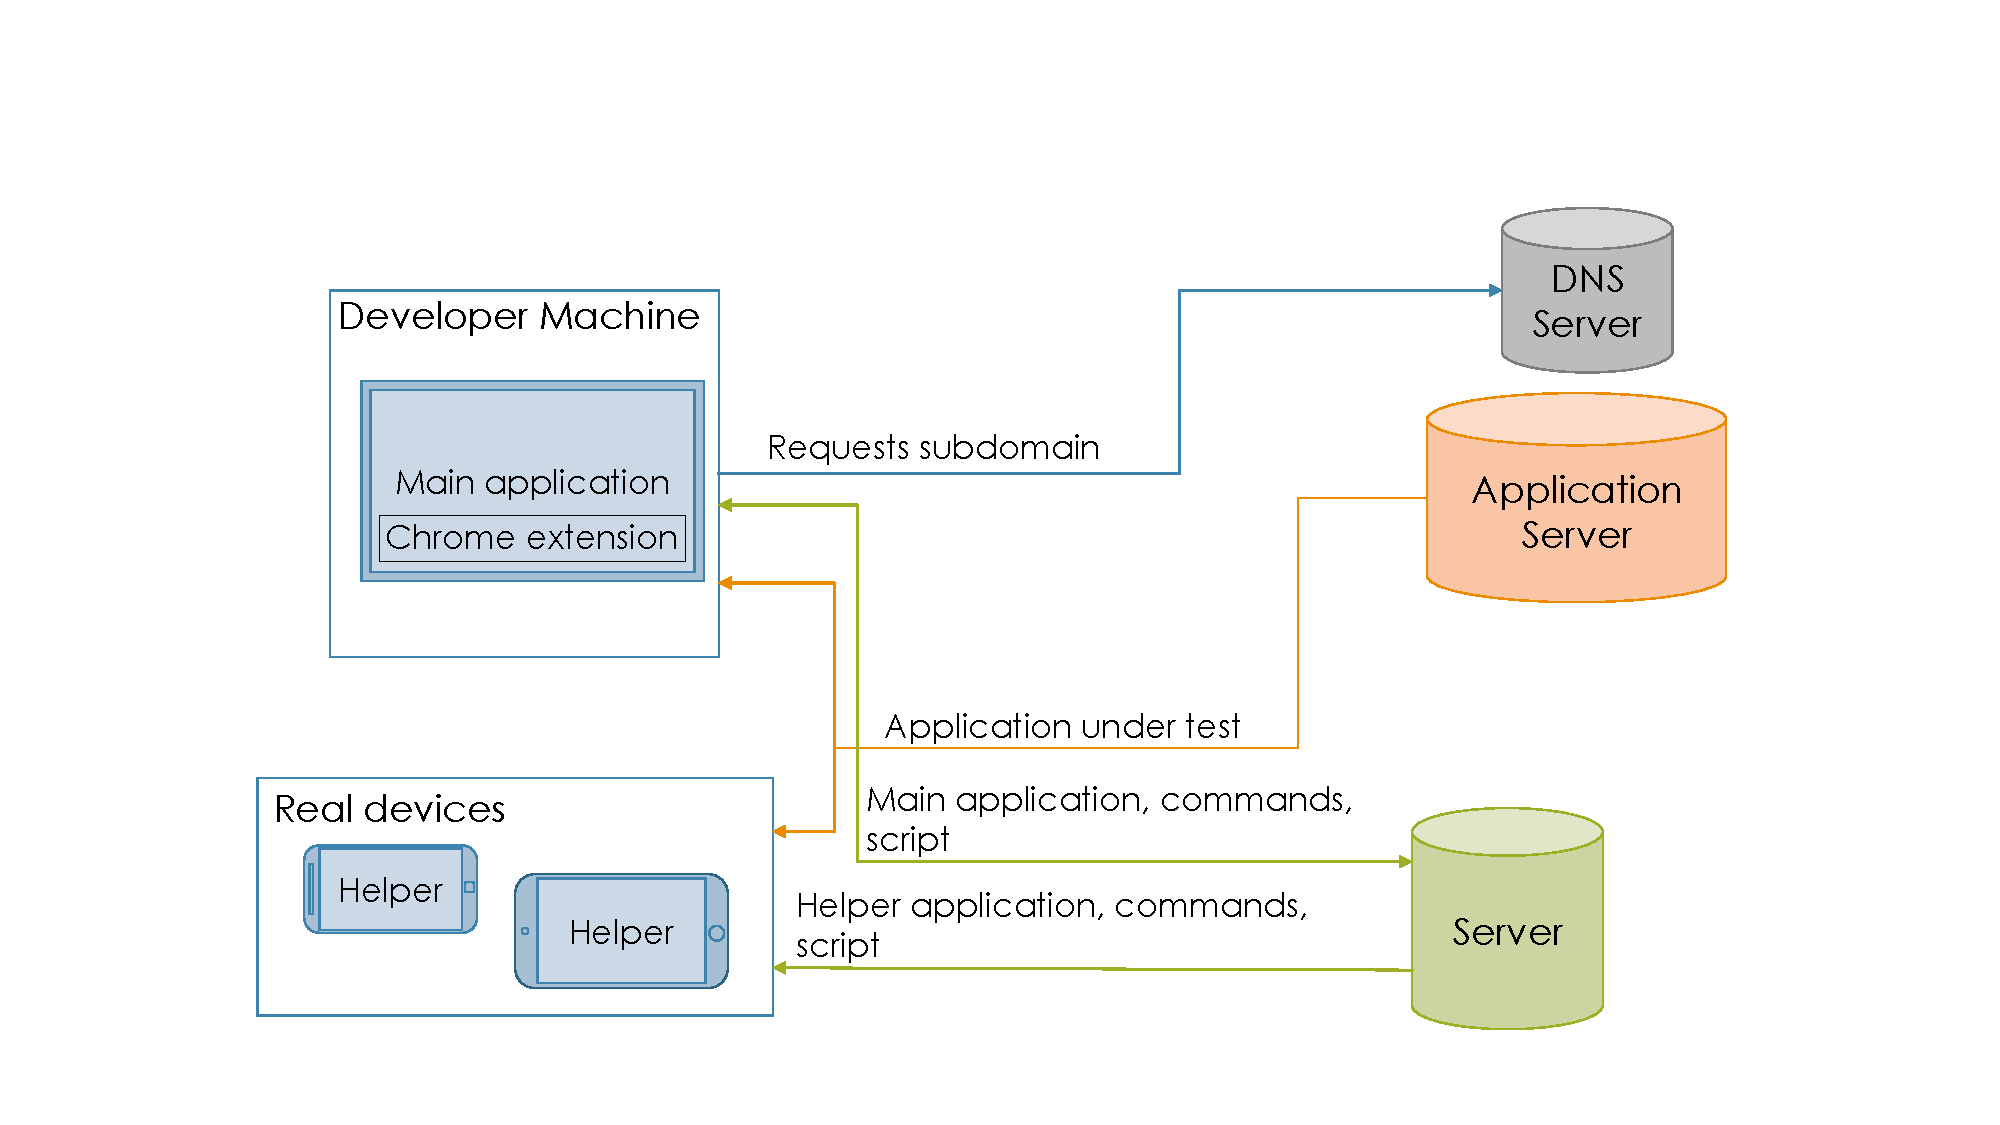
\includegraphics[width=0.85\textwidth]{images/architecture_2.pdf}
	\caption[Architecture of XDTools]{Architecture of XDTools}
	\label{fig:architecture}
\end{figure}

Additionally, a local DNS server runs on the developer's machine. It is responsible for creating different subdomains for the emulated devices. The DNS server is required for properly testing and debugging on emulated devices, but if only real devices are used, it is not needed and can be disabled in the options of XDTools.

Furthermore, a Chrome extension runs in the browser of the developer's machine. This extension is needed for function debugging and inspection as well as HTML inspection. The Chrome extension communicates with the main application via the server.

Finally, some web server needs to provide the application under test. However, any web server can be used and XDTools does not place any restrictions. The only requirement is that the developer injects a small script that is hosted on our server at the top of each HTML page of the application. The script is responsible for performing many actions that would otherwise be difficult, such as executing JavaScript, recording events and adding CSS to the application under test.

\section{Choice of Technologies}

Since XDTools includes desktop devices as well as mobile devices, it should be platform-independent. Thus, XDTools is implemented using standard web technologies, i.e. HTML5, CSS3 and JavaScript. This allows XDTools to be run in any modern web browser without requiring installation of any additional software. The fact that we focus on web-based cross-device applications only makes web technologies even more suited for XDTools. XDTools does not rely on any database, instead HTML5 Local Storage\footnote{\url{http://www.w3schools.com/html/html5_webstorage.asp}} is used for the data that we want to store. XDTools only need to store three things:
\begin{itemize}
	\item Custom devices for emulation that were added by the developer.
	\item Device configurations.
	\item Event sequences for replaying.
\end{itemize}
All those things only need to be accessed by the developer that created them. Thus, it makes sense to only store the data locally. Furthermore, the amount of data that needs to be stored is rather low. 

\subsection{Server Side}

On the server side, XDTools uses Node.js\footnote{\url{https://nodejs.org/en/}}. Node.js is a JavaScript runtime that uses asynchronous I/O with an event-driven programming model. It is lightweight and scales well with a large number of connections. Furthermore, it has the advantage that both the client and server side are implemented using JavaScript. Thus, no data conversions are required. In XDTools, fast communication between the PC and the connected real devices is required and Node.js fulfills this requirement. Node.js' package ecosystem, npm\footnote{\url{https://www.npmjs.com/}}, provides a large number of modules which extend the capabilities of Node.js. XDTools uses the following modules: 
\begin{itemize}
	\item Express\footnote{\url{http://expressjs.com/}}: Express is a minimal and flexible web application framework that provides a set of features for web and mobile applications. In XDTools, Express is responsible for serving the content to the clients.
	\item shortid\footnote{\url{https://github.com/dylang/shortid}}: shortid generates short URL-friendly unique IDs and is responsible for generating the device IDs for the emulated and real devices in XDTools. As each emulated device gets a subdomain based on its ID, shortid is ideal for our purpose.
	\item Socket.IO\footnote{\url{http://socket.io/}}: Socket.IO enables real-time bidirectional event-based communication. If available, it uses HTML5 WebSockets, otherwise it uses fallback mechanism like AJAX\footnote{\url{http://www.w3schools.com/ajax/}} long-polling. In XDTools, Socket.io is used for the communication between the server and clients.
\end{itemize}

Socket.io is better suited for XDTools than AJAX for multiple reasons: First, we need to be able to send push data to clients from the server when sending commands to devices and AJAX is intended to allow clients to pull data from the server. Also, data transfer with AJAX comes with a significant overhead because HTTP headers are transmitted with each piece of data. As we mentioned before, fast communication between the server and the devices is a requirement for XDTools and AJAX would not fulfill this requirement sufficiently. However, AJAX is used for communicating with the DNS server.

\subsubsection{DNS Server}

XDTools requires a DNS server for registering subdomains for the emulated devices. It should be easy to dynamically register new subdomains to the DNS server. Furthermore, the DNS server should forward any unknown domains to the standard DNS server. rainbow-dns\footnote{\url{https://github.com/asbjornenge/rainbow-dns}} fulfills both those requirements. It is a Node.js-based DNS server with an HTTP API that makes it trivial to register new domains from the main application of XDTools. When starting the server, the IP address of the standard DNS server can be passed as an argument, allowing rainbow-dns to forward unknown domains to the standard DNS server.

\subsection{Client Side}

The client side of XDTools is implemented using JavaScript with jQuery\footnote{\url{https://jquery.com/}}. jQuery allows easy selection and modification of HTML elements as well as easy event handling, features that are crucial to XDTools. As an additional helper, we use jQuery UI\footnote{\url{https://jqueryui.com/}}. jQuery UI is mainly used for the autocomplete functionality provided in several places and for easy resizing of the individual interface components of XDTools. It is also used for resizing the emulated devices to change their resolution. The Twitter Bootstrap\footnote{\url{http://getbootstrap.com/}} framework is used to give XDTools a nice and uniform look-and-feel. It is also used for facilitating the implementation of things like modal boxes and tabs. 

XDTools uses QR codes for connecting real devices to the server. We use the jQuery-based QR Code library jQuery.qrcode\footnote{\url{https://larsjung.de/jquery-qrcode/}} for generating those QR codes. Using jQuery selectors, the content of an HTML element can be set to a QR code with the desired content and size.

HTML5 Drag and Drop\footnote{\url{http://www.w3schools.com/html/html5_draganddrop.asp}} is used for accurate positioning of devices and timing of event sequences. HTML5 \lstinline|postMessage| is used for communication between the application under test and XDTools. Thus, no additional library for communication is needed inside the application under test.

The script that is injected into the application under test is implemented in pure JavaScript. Using libraries like jQuery inside this script could lead to conflicts with other libraries included in the application under test or different versions of jQuery. Also, loading jQuery into the application creates some additional overhead and might not be what the developer of the application wants.

The Chrome DevTools extension is implemented using JavaScript. It uses the Command Line API\footnote{\url{https://developer.chrome.com/devtools/docs/console-api}} for accessing the functions needed to inspect HTML, debug functions, and more. The extension uses Socket.IO for communicating with the server. 

\section{Emulation of Multiple Devices}

Devices are emulated using \lstinline|iframes|: Each emulated device is represented by its own \lstinline|iframe| that loads the application under test. However, loading the same domain inside multiple \lstinline|iframes| would lead to the sharing of local resources between emulated devices.  In order to prevent this, a unique subdomain based on the ID of the device is registered with the local DNS server. All subdomains point to the application under test, but as the application is accessed through different domains, no local resources are shared between the emulated devices. Domains that are unknown to the local DNS server are forwarded to the standard DNS server. 

The resolution of each \lstinline|iframe| corresponds to the resolution of the device that it represents in CSS pixels. Currently, only the resolution of the target devices is emulated, but in the future, XDTools could be extended to support emulation of other aspects. The scaling of the device is set using the CSS property ``transform'', e.g. by setting ``transform: scale(0.5)'' to scale a device to half its usual size. Using the ``transform'' property does not change the resolution of the \lstinline|iframe| of the emulated device, only the screen space that the \lstinline|iframe| occupies. Thus, the layout of the emulated device remains intact even if it is scaled down. If the developer instead wants to change the resolution of a device, they can click on the bottom-right corner of the \lstinline|iframe| and drag to increase or decrease the resolution. 

The devices can be moved around using HTML5 Drag and Drop. However, we cannot just make the devices \lstinline|draggable| by default. The developer should not be able to move the device if they click on the \lstinline|iframe| because otherwise interaction with the \lstinline|iframe| would be restricted. Thus, we chose to only make devices \lstinline|draggable| if the developer clicks on the header of the device. For this reason, we assign a click handler to each device that checks if the developer clicked on the header of the device. If yes, we make the device \lstinline|draggable|. 

When the developer starts dragging the device, the device ID is assigned as data to the event. However, the device ID is not the only required data. If the developer drags the device to a certain position, we cannot just assign this position to the device. If we did, the top left corner of the device would be at the position where the device was dropped, but the developer probably did not click on the top left corner of the device when they started dragging it. Thus, we need to compute the offset of the click from the top left corner of the device and adjust the position accordingly when the device is dropped. For example, if the developer clicks on the device 10 pixels from the top and drops the device x pixels from the top of the device area, we need to assign the position x - 10. For achieving this, we compute the offset when the developer clicks on the header of the device and set the offset as data to the event.

\subsection{Color Generation}

The primary goal of the device colors was to make it easy to distinguish devices, thus their colors should be as distinct as possible. For achieving this, we use the HSL color space\footnote{\url{https://en.wikipedia.org/wiki/HSL_and_HSV}}. Finding distinct colors is a much simpler task in the HSL color space compared to the RGB color space because only one of the three color components has to be modified. In the HSL color space, colors consist of the three values hue, saturation and lightness. The colors of the devices should all have the same saturation and lightness, thus the only value that needs to be determined is the hue. The hue can have any value between 0 and 360. Since our goal is to have colors that are easily distinguishable, their hues should be as different as possible. A simple algorithm can be used for determining the color of the next device:
\begin{enumerate}
	\item If no colors have been assigned yet, assign the color 0/360.
	\item If only one color has been assigned, assign the color 180.
	\item If at least two colors have been assigned: Order the assigned colors by their values, compute the maximum distance between any two neighboring colors and assign the color in-between.
\end{enumerate}

\section{Easy Integration of Real Devices}

Real devices can be connected by scanning a QR code or opening a URL. When the URL is opened, the device loads the helper application. Once the helper application is loaded, the application under test is shown in a full-screen \lstinline|iframe| on the device. If the developer issues any command in the main application, e.g. refreshing the \lstinline|iframe| of the real device, the command is first sent to the server and then forwarded to the target device. 

\section{Easy Switching of Device Configurations}

Device configurations are stored in Local Storage. The Local Storage stores an array containing the names of all saved device configurations. This array is used for the autocomplete functionality and for retrieving the actual device configuration, an array of devices. For each device, the name, width, height, device pixel ratio, scaling, layer and position is stored. It does not make any sense to store real devices because they might not be available when the device configuration is loaded and they need to be re-connected manually anyway by opening the appropriate URL, thus only emulated devices are stored in device configurations. If the developer wants to load a device configuration, an ID is requested for each device, then the device is created and its scaling and position are set according to the values in the Local Storage.

\section{Integration with Debugging Tools}

The following subsections describe the implementation of the parts that were adopted from the browser's debugging tools and extended.

\subsection{Shared JavaScript Console}

The following types of logging messages are aggregated in the shared JavaScript console:
\begin{itemize}
	\item \lstinline|console.log|
	\item \lstinline|console.debug|
	\item \lstinline|console.warn|
	\item \lstinline|console.info|
	\item \lstinline|console.error|
	\item \lstinline|console.count|
	\item \lstinline|console.dir|
	\item \lstinline|console.assert|
\end{itemize}
In the script that is injected into the application under test, those functions are overwritten by a new function and the original functions are stored. The new function performs the following two actions: First, it sends the content and type of the logging message to our server. Second, it calls the original logging function. Thus, the logging messages are still displayed in the browser console, but forwarded to our console in addition.

Forwarding JavaScript errors is implemented by assigning an event handler to JavaScript errors using \lstinline|window.onerror|. Whenever a JavaScript error occurs, the event handler is called. Inside the event handler, the JavaScript error message is sent to our server, together with the stack trace if available. 

Commands that are sent to devices are executed by calling \lstinline|eval| with the command string as argument.

\subsection{Function Debugging and Inspection}

Function debugging and inspection requires the Chrome extension. When the developer adds a new function to debug, a command is sent to each activated emulated device. If a device receives the name of a function to debug, it overwrites the function to debug by a new function and stores the original function. The overwriting function performs the following actions:
\begin{enumerate}
	\item It highlights the device with a semi-transparent green overlay.
	\item It calls the original function and stores the return value.
	\item It removes the highlighting.
	\item It returns the return value.
\end{enumerate}
After overwriting the original function, the device sends a message back to the main application that it is ready for debugging. The main application then sends a command to the Chrome extension with the name of the variable that stores the original function, together with the URL of the \lstinline|iframe| of that device. The Chrome extension then calls the ``debug'' function with the function name and the URL of the frame that represents the device.

If the developer is done debugging a function, they can remove it from the list of debugged functions and the original function is restored inside the script. Then, a command is sent to the DevTools extension, informing it to stop debugging the function. 

The functions that are debugged run inside an \lstinline|iframe| and the URL of the \lstinline|iframe| needs to be passed as a parameter. However, when a new device is added, the hook for the \lstinline|iframe| of the new device does not exist yet and the Chrome DevTools need to be closed and re-opened. Similarly, if the URL of a device changes, the hook is lost. Unfortunately, there is no way of automatically re-opening the DevTools. For this reason, a red overlay containing a warning text is shown whenever a URL changes or a new device is added. The warning can be seen in Figure~\ref{fig:warning}.

\begin{figure}[H]
  \centering
    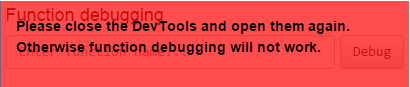
\includegraphics[width=0.6\textwidth]{images/screenshots/warning.png}
	\caption[Screenshot: Function debugging warning]{Warning that is shown for function debugging}
	\label{fig:warning}
\end{figure}

\subsection{HTML Inspection}

HTML inspection also requires the Chrome extension and thus only works on emulated devices. If the button to inspect the HTML is clicked, a command is sent to the DevTools extension, telling it to open the \lstinline|body| element of the frame with the URL of the device. The HTML inspection view in the Chrome DevTools then jumps directly to the body of the HTML of the device.

\subsection{Shared CSS Editor}

Inside the injected script in the application under test, a stylesheet is created and added to the DOM tree. Whenever the developer adds a new rule to the CSS editor, a command is sent to all active devices and the rule is added to an array containing all CSS rules. Whenever the array with the CSS rules changes, the stylesheet is rewritten. Retrieving the appropriate rule from the stylesheet and modifying it is difficult and time-consuming, simply rewriting the stylesheet is much more convenient, especially since we do not expect developers to add hundreds of rules to the shared CSS editor. If a rule is disabled, it is removed from the stylesheet; if it is enabled again, it is re-added to the stylesheet.

For the CSS autocomplete functionality, we need to get all available CSS properties. The available CSS properties are retrieved using \lstinline|document.body.style| which contains all available CSS properties, even if they are not set. The CSS properties of \lstinline|document.body.style| are then converted to an array of available CSS properties.

\section{Automatic Connection Management}

In the script that is injected into the application under test, a connection function is available. When a device wants to connect to another device, a command is sent to that device. That device then calls the connection function. The connection function returns the URL that has to be loaded to connect the device. The URL is then loaded on the device that wants to connect.

The connection function has to be modified by the developer such that it returns the appropriate URL.

\section{Coordinated Record and Replay}

Recording interactions is done by assigning event handlers for all events that we want to record. It is important that no other script receives the events before us, because otherwise they could modify the page or even stop event propagation. For this reason, the event handlers are assigned as soon as the injected script is loaded and the script has to be placed at the top of the page. However, the event handlers do not do anything as long as recording has not started yet. When the developer starts recording, all events are logged to an array. After finishing recording, all circular structures are removed. All other event properties are kept so the events can be replayed accurately. The array of events is then sent to the main application. 

Furthermore, all event handlers are capturing and are assigned to the \lstinline|document| itself. Since no other element in the DOM hierarchy can be above the \lstinline|document| element, the \lstinline|document| element is always the first element that receives an event with capturing event handlers. 

The event sequences should be replayable on other devices than the recording device, therefore some way of determining the target of the event is required. Whenever an event handler is triggered, the DOM hierarchy is traveled up from the target of the event until an ID is encountered. Accessing this ID first, we can determine the target element by taking the appropriate child until the target element is reached. From this, we can derive a hierarchy that describes how to reach the target element on a device and replaying the event on another device becomes possible.

When visualizing event sequences, each event requires some space. Thus, events that happen close together in time are grouped together. If events were not grouped, the visualization of the event sequence would not represent the true timing of the events: Even though two events might occur almost simultaneously, they would both require some space when visualized and thus give the impression that some time passed between them. The following algorithm is used for grouping events:
\begin{enumerate}
	\item Take the first unprocessed event.
	\item Take all events that happen within x milliseconds of that event and group them together.
	\item Visualize the grouping of events.
	\item Go to Step 1.
\end{enumerate}

When the developer starts replaying, the event sequences assigned to a device are sent to that device along with the list of breakpoints. The events that happen before the first breakpoint are then triggered using \lstinline|setTimeout|. After all events have been triggered, a message is sent to the main application, telling it that a breakpoint has been reached. After the developer chooses to continue, a message is sent to all replaying devices telling them to continue.

When replaying events, the target element of an event is determined using the hierarchy computed when recording. All events are replayed using the properties recorded in the event sequences. For most events, replaying with the properties logged when recording is enough for realistically reproducing the events. However, some events require a bit more work. Replaying key events is possible, but no text is written into input fields. In addition to the key events, we also need to trigger a text event using the correct char code. Scrolling events also do not scroll. Thus, we also log the scrolling position after a scrolling event occurs and manually set it after replaying the event. Furthermore, the backspace key cannot be reproduced with neither text events nor key events. Thus, we manually determine the position of the caret if the backspace key is pressed and delete the last character before the caret when replaying. 

\section{Integration with Polymer and Shadow DOM}

Although XDTools works with all web-based cross-device applications, one of the initial goals was to make it work with applications developed with XD-MVC. XD-MVC can either just be used as a JavaScript API or it can be used together with Polymer. Polymer provides developers with the option to use Shadow DOM\footnote{\url{http://www.w3.org/TR/shadow-dom/}}. Shadow DOM refers to the ability of the browser to include a subtree of DOM elements into the rendering of the document, but not into the main document tree. Thus, it can encapsulate components and prevent them from being reached by traditional tree walking functions such as \lstinline|childNodes| and \lstinline|firstChild|. We must assume that some applications implemented with XD-MVC use Polymer and Shadow DOM and XDTools should support those applications as well. However, a few modifications are required for supporting both Polymer and Shadow DOM. First, determining the target of an event can become more difficult because the element might not be accessible from the global scope. Second, debugging functions that are not accessible from the global scope should be possible and we need some way of accessing those functions. Furthermore, we want to be able to add CSS to elements that are not accessible from the global scope.

\subsection{Determining Event Targets}

An element can define Shadow DOM by attaching a shadow root to itself. The Shadow DOM can be accessed using the \lstinline|shadowRoot| property of the element. Without Shadow DOM, finding the nearest element with an ID was enough for determining the path that leads to the target element of an event. With Shadow DOM, we need to additionally consider all shadow roots that lead from the \lstinline|body| element to the target element. The \lstinline|path| property of the event contains all elements that were visited by the event. We adjusted our algorithm in the following way:
\begin{enumerate}
	\item Take the lowest (in the DOM hierarchy) element in the \lstinline|path| that has not yet been processed.
	\item Determine how to reach this element from the next higher element in the path:
	\begin{enumerate}
		\item Check if the element has a parent node. If not, it must be the hierarchically highest element inside a shadow root. Thus, it can be reached by accessing the \lstinline|shadowRoot| property of the higher element.
		\item Check if the element has an ID. If yes, it can be reached using the ID.
		\item If the element has a parent element but no ID, it can be accessed by accessing the appropriate child of the parent element.
	\end{enumerate}
	\item Go back to Step 1.
\end{enumerate}
Using this hierarchy, the target element can already be reached, but because of elements with ID, some steps can be skipped. Inside each shadow root, we look for the lowest element with an ID. All elements inside the shadow root but above that element can be skipped and the ID can be accessed directly. If no element has an ID, we have to keep all elements. The same can be done for the path from the \lstinline|body| element to the highest shadow root and for the path from the lowest shadow root to the target element. Using this algorithm, the shortest path to the target element is computed. For applications that do not contain any Shadow DOM, the algorithm yields the same result as the standard algorithm described earlier. The computed hierarchy can be used to determine the target of the event on other devices by accessing shadow roots instead of IDs or children when appropriate.

This modified algorithm allows us to record and replay events on applications that use Shadow DOM. 

\subsection{Determining Scopes}

There are two things to be considered: First, there may be shadow roots in the application. Second, the developer can define functions for their custom Polymer elements that need to be accessed using the Polymer element. In principle, those functions can be accessed using the appropriate path through the DOM tree, but determining this path is not trivial. Thus, we want to automatically determine all different scopes on which functions can be defined, i.e. all shadow roots and Polymer elements and the path through the DOM tree that leads to those scopes. We implemented the following algorithm for determining the scopes:
\begin{enumerate}
	\item Add the \lstinline|body| element to the processing queue.
	\item As long as the processing queue is not empty, take the first element and perform the following actions:
	\begin{enumerate}
		\item If the element has the property \lstinline|shadowRoot|, we found a new scope and add it to the list of scopes, together with the path that determines how to reach the scope. Then we add the shadow root of the element to the processing queue.
		\item If the element has the property \lstinline|is|, it is a Polymer element and we add it to the list of scopes, together with the path. Then we add each child of the element to the processing queue.
		\item If neither of the above is true, we have not found a new scope and we simply add all children of the element to the processing queue.
	\end{enumerate}
\end{enumerate}
When the algorithm has finished, the list of scopes is sent to the main application. In the main application, the developer can choose the scope that they want to work with from a drop-down menu.

The selected scope has an influence on the following three components of XDTools:
\begin{itemize}
	\item Shared JavaScript console: In the shared JavaScript console, all commands in the console are executed in the selected scope. 
	\item Shared CSS editor: In the CSS editor, the CSS rule is added to the selected scope. Each scope has its own stylesheet containing the CSS rules for that scope.
	\item Function debugging: The functions that are debugged are on the selected scope.
\end{itemize}
In addition, the developer can directly jump into the HTML of each scope by clicking the HTML inspection button and choosing the scope from a drop-down menu.